%% ==============================
% Part is used only in PhD thesis
\part{The Implementation}
\chapter{\iflanguage{ngerman}{Implementierung}{Implementation}}
\label{sec:implementation}

\section{Preparation Work}
The concept should be tested with real hardware at the described in \autoref{c3_sec_used_robots}. The used hardware are KUKA robots and communication with the robots is done via \gls{rsi}. There existed an old driver for the \gls{rsi} as well as a repository with the description of the used robot models.
\subsection{Porting of the KUKA RSI to \gls{ros2} Rolling}
The existing driver for the \gls{rsi} was only available for older versions of \gls{ros2} and needed to be ported. 
The driver is implemented as a system and the interfaces of the driver had to be adapted to the signature used in \gls{ros2} Rolling. After the adaption, the drivers were tested with the robots and some issues were found which needed fixing.\newline 
The first issue discovered was timing related. The control loop of the standard control node in \gls{r2c} consists roughly of five steps, as listed in the following:\newline
\lstset{language=C++,basicstyle=\small}
\begin{lstlisting}[caption=Pseudo code for the control loop.,label=c5_code_control_loop]
// creat controller manager with an rclcpp::executor
auto cm = 
    std::make_shared<controller_manager::ControllerManager>
        (executor, cm_node_name);
while (rclcpp::ok())
{   
    // step 1: calculated meassured_period
    // Call read in RSI driver, which is blocking
    cm->read(cm->now(), measured_period); // step 2: BLOCKING 
    cm->update(cm->now(), measured_period); // step 3
    cm->write(cm->now(), measured_period); // step 4
    //step 5 sleep until next iteration
}
\end{lstlisting}
The communication with the robot controller needs to be precisely timed. The driver creates a UDP server and communicates with the controller of the robot via UDP messages. However, reading the new arrived messages from the UDP server (step 2 in \autoref{c5_code_control_loop}), is blocking. This leads to driver blocking if no new messages have arrived. Therefore, the update rate set for the control node can get messed up, since the blocking read is not preempted. This ultimately leads to the robot controller ending the connection. This problem occurs especially if no real-time kernel is used.\newline
As solution, for the communication with the robot controller the sleep in the control node (step 5 in \autoref{c5_code_control_loop}) is omitted. The synchronization between the robot controller and the controller manager is done via the incoming messages of the robot controller, which acts as clock generator.

A second issue discovered was that the default clock used for the control node does not provide a monotonic increasing time. On platforms where no real-time kernel is installed and especially on embedded devices, this leads to issues. For example, if the time does not increase monotonically, the trajectory generated by the \textit{JointTrajectoryController} includes jumps, which leads to the velocity of the robot's joints exceeding the velocity limits. As a solution, the control node is started with a clock where the time is incremented in monotonic steps as shown in \autoref{c5_code_monotonic_time}.
\lstset{language=C++,basicstyle=\small}
\begin{lstlisting}[caption=Small code extract for setting monotonic clock.,label=c5_code_monotonic_time]
rclcpp::NodeOptions node_options;
node_options.clock_type(rcl_clock_type_t::RCL_STEADY_TIME);
// creat controller manager with an rclcpp::executor
auto cm = std::make_shared<
            controller_manager::ControllerManager>(
                executor,
                cm_node_name, node_options);
 // control loop
\end{lstlisting}

\subsection{Restructuring of the \textit{kuka\_experimental} Repo}
The ported \gls{rsi} drivers have then been added to the \textit{kuka\_experimental} repository, which includes the description files of the used robots. The descriptions were updated to include parameters to pass the IP address and port to the driver. Additionally, some restructuring was done to ease the selection and starting of the correct description files.

\section{Adaptions in the \gls{r2c} Framework}
In order to support distributed control of multiple robots in \gls{r2c}, a few changes had to be implemented. In the following, first some preliminary changes are introduced which provide the basis for implementing the proposed concept. Then the changes of the \glspl{handle} and how the controller manager has been adapted are presented.

\subsection{Allow to Start with an Empty Robot Description File}
The description of the hardware, including which \glspl{ci} and \glspl{si} are provided, is normally described in a '\texttt{.xacro}' file. This file is then passed to the controller manager, parsed and the \glspl{ci} and \gls{si} are exported by the hardware. 
As described in \autoref{sec:concept}, a central controller manager does not need to have its own hardware. It imports the \glspl{ci}, \glspl{si} and \glspl{ri} of the sub-controller managers. The problem is, that in \gls{r2c} a controller manager must have its own hardware. In addition, it is not possible to pass the robot description file to the controller manager other than via file at startup. In a distributed setting, it would be an advantage to start a sub-controller manager and then pass the description of the hardware later so that the system is more flexible. \newline
Consequently, the controller manager was changed to allow passing an empty robot description file. The change includes the possibility to pass the robot description file over the \textit{~/robot\_description} topic. At construction time, it is checked if the robot description file passed to the controller manager is empty. If no robot description is passed via file, the construction of the controller manager is continued without initializing of the resource manager. The controller manager instead subscribes to the \textit{~/robot\_description} topic relative to its own private namespaces. This is done to avoid clashes if multiple controller managers are present. Each of the controller managers could possibly get different hardware passed. The subscription is set to \textit{transient\_local} which is similar to "latching" publishers in \gls{ros}. This is needed, so that a late joining controller manager still gets the description when it is published, before the controller manager can subscribe to the topic. A code small snippet is presented in \autoref{c5_code_robot_description}.
\lstset{language=C++,basicstyle=\small}
\begin{lstlisting}[caption=Small code snippet for usage of the robot\_description topic.,label=c5_code_robot_description]
// ControllerManager constructor
{   
...
  if(robot_description.empty()) {
    create_subscription<std_msgs::msg::String>(
      "~/robot_description",
      rclcpp::QoS(1).transient_local(),
      std::bind(&ControllerManager::robot_description_callback,
        this, std::placeholders::_1));
    } 
...
}
// robot_description_callback()
{
    // check if have been called
    if(!resource_manager->is_urdf_already_loaded()) 
        // if not: get urdf, parse, and initialize
}
\end{lstlisting}

\subsection{Activation of Hardware}
After the robot description file has been parsed and the resource manager initialized, the hardware is either configured or automatically activated by default. There was no way to configure or activate the hardware components later or at a specific time. In a distributed setting, this can potentially lead to issues, as a sub-controller manager would instantly activate and start to communicating with its hardware. However, this should only be done after the sub-controller manager has registered with the central controller manager.\newline
In order to change this, a hardware spawner is introduced. The hardware spawner is a standalone executable which acts as interface for the \lstset{language=C++,basicstyle=\small\ttfamily}\lstinline{~/set_hardware_component_state} service of the controller manager. It interfaces the service call and allows configuring or activating a hardware component after the resource manager has been initialized and the \glspl{ci} and \glspl{si} have been imported into the resource storage. This way a sub-controller manager can be initialized. Then the \glspl{ci} and \glspl{si} can be created and registered at the central controller. Then the hardware component can be configured or activated at a later point and communication with the real hardware is started.\newline
The activation can then either be done directly in the Python launch file as shown in \autoref{c5_code_hardware_spawning_launch} or via the command line as shown in the \autoref{c5_code_hardware_spawning_cli}. Both examples show the activation of a
\lstset{language=Python,basicstyle=\small}
\begin{lstlisting}[caption=Example of using the hardware spawner in a python launch file.,label=c5_code_hardware_spawning_launch]
    hardware_activation = Node(
        package="controller_manager",
        executable="hardware_spawner",
        arguments=["ComponentName", "--activate"],
    )
\end{lstlisting}
fictional hardware component called 'ComponentName'. With the Python launch file, the old behavior can be mimicked by  'automatically' configuring or activating the hardware component at the launch time. In addition, other nodes can be started in a timed manner depending on when the hardware was successfully activated. This was previously not possible. On the other hand, the hardware can be activated manually from the command line, which was not possible either.
\lstset{
    basicstyle=\fontsize{10}{12}\ttfamily,
    columns=fullflexible,
    language=bash,
    breaklines=true
}
\begin{lstlisting}[caption=Example of using the hardware spawner from command line., label=c5_code_hardware_spawning_cli]
ros2 run controller_manager haelware_spawner "ComponentName" 
    --activate
\end{lstlisting}

\subsection{Chainable Joint Trajectory Controller}
In order to test the concept of distributed chained controllers, the \textit{JointTrajectoryController} needed to be chainable. For this, the \textit{JointTrajectoryController} now inherits from the \textit{ChainableControllerInterface}. The controller now can be set to chained mode. On setting the chained mode, the controller creates and exports \glspl{ri} for each of the joint's position, velocity, acceleration and effort \gls{ci}, it controls.\newline
\lstset{language=C++,basicstyle=\small}
\begin{lstlisting}[caption=Update function for \textit{ChainableControllerInterface}.,label=c5_code_chainable_update]
return_type ChainableControllerInterface::update(
  const rclcpp::Time & time, const rclcpp::Duration & period)
{
  return_type ret = return_type::ERROR;
  if (!is_in_chained_mode())
  {
    ret = update_reference_from_subscribers(time, period);
    if (ret != return_type::OK)
    {
      return ret;
    }
  }
  ret = update_and_write_commands(time, period);
  return ret;
}
\end{lstlisting}
One thing that had to be considered was that for a chained controller that is not in chained mode, the \lstset{language=C++,basicstyle=\small\ttfamily}\lstinline{update(time, period)} function calls the \lstset{language=C++,basicstyle=\small\ttfamily}\lstinline{update_and_write_commands(...)} function before writing the commands. Like the name suggests, in this case the \glspl{ri} are updated locally with the contents from the subscribers instead of being set externally by a chained controller. This is illustrated in \autoref{c5_code_chainable_update}. However, for the \textit{JointTrajectoryController} this leads to a problem. A chained controller expects one \gls{ri} per each \gls{ci} the \textit{JointTrajectoryController} has. On the other hand, if the \glspl{ri} are updated by the \textit{JointTrajectory Message} of a publisher subscribed to, this message can contain multiple \textit{JointTrajectoryPoint} points. As a result, the \gls{ri} would need to be multidimensional. \newline
As a workaround, instead of updating the \gls{ri} in the \lstset{language=C++,basicstyle=\small\ttfamily, breaklines=true}\lstinline{update_reference _from_subscribers(...)} function, it is now checked at one place inside the function \lstset{language=C++,basicstyle=\small\ttfamily}\lstinline{update_and_write_commands(...)} if the controller is in chained mode or not. If the chained mode is enabled, then a new \textit{JointTrajectory Message} is created from the \glspl{ri} and used for calculating the trajectory. Otherwise, the \textit{JointTrajectory Message} is directly taken from the publishers.

\subsection{Adaption of the Handles}
As described in \autoref{c4_sec_adaption_of_handles} the \glspl{handle} are the point where the system was split. One problem that arose here was that the \glspl{handle} only store a pointer to memory allocated in the hardware, instead of allocating the memory locally, see \autoref{c3_sec_link_ctrl_hw}. Therefore, neither a \gls{si} nor a \gls{ci} can know when the value has been changed by the hardware. This poses a problem as in the distributed case the value stored in the \gls{handle} should be published on changed. There are two different ways to approach this, each with its own advantages and disadvantages. The first approach was to publish the value of the \gls{handle} timer-based periodically. With this approach, the creation of the \glspl{handle} in the hardware can stay the same. \autoref{c5_fig_handle_uml} displays the adapted class hierarchy as well as the newly introduced distributed \glspl{handle}. The former base class \textit{ReadOnlyHandle} has been replaced by a \textit{HandleInterface}, \textit{ReadHandleInterface} and a \textit{WriteHandleInterface}. This has been done in order to have a clear separation of readable and writable \glspl{handle}. The \textit{HandleInterface} is the base class for all \glspl{handle} and contains basic functionality like getting a full qualified name, namespace and the like. In addition, the pointer to the value stored inside the hardware, is stored here. The \textit{ReadHandleInterface} ensures that all readable \glspl{handle} implement the \textit{get\_value()} function for retrieving the stored value of the pointer. The \textit{WriteHandleInterface} on the other hand, ensures that all writable \glspl{handle} have a \textit{set\_value()} function for commanding the \textit{handle}. \newline
With this class hierarchy, the \textit{ReadOnlyHandle} is only the base class of readable \glspl{handle} and not of all \glspl{handle} as before. The same applies for the \textit{ReadWriteHandle}. Next, the \textit{DistributedReadOnlyHandle} and \textit{DistributedReadWriteHandle} as well as their subclasses \textit{DistributedStateInterface} and \textit{DistributedCommandInterface} were introduced. This change allows using shared pointers inside the resource storage and setting the type for the \glspl{si} to \textit{ReadOnlyHandle} and \textit{ReadWriteHandle} for the \glspl{ci}. Then at runtime we can either store a \gls{si} or a distributed \gls{si} and the correct \lstset{language=C++,basicstyle=\small\ttfamily}\lstinline{get_value()} function is called via dynamic binding. The same applies for the \gls{ci} and distributed \gls{ci}. \newline
The newly introduced distributed \glspl{handle} are used by the central controller. The central controller creates them and stores them inside its resource storage. Controllers can then claim them as they would with any \gls{ci} or \gls{si} interface. The only difference is that for a distributed \gls{handle} the value is received over a \gls{ros2} topic from the counterpart on the sub-controller manger site and then stored inside the \gls{handle}. If a controller writes a command to a distributed \gls{ci} the value is immediately published. \newline
\begin{figure}[htbp]
	\centering
	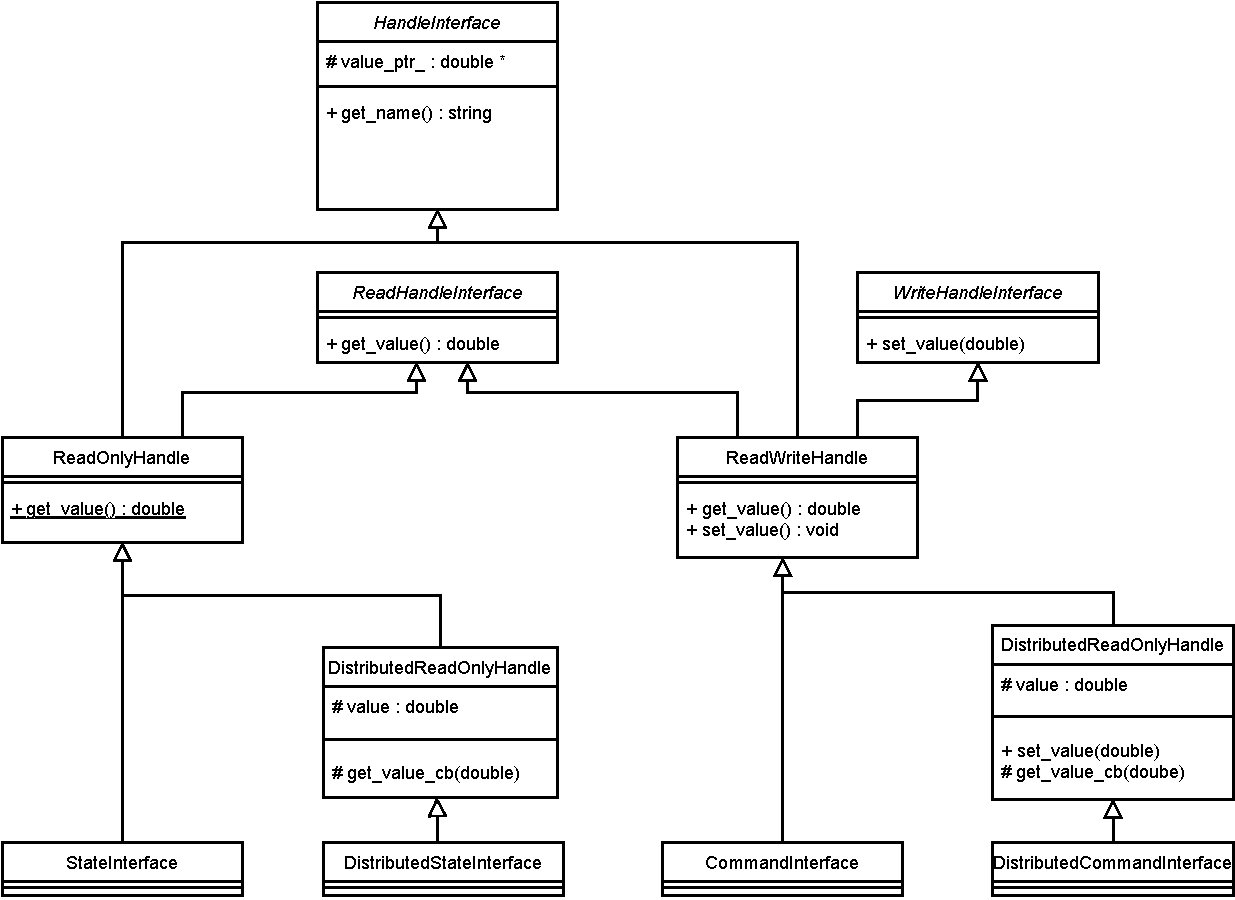
\includegraphics[width=1\textwidth]{Figures/c5/Handles_UML.pdf}
	\caption{UML class diagram of the different \gls{handle} types, including the newly introduced distributed \glspl{handle}. One should note that the UML class diagram does not contain every member and function of the classes, but only shows the most important parts. }
	\label{c5_fig_handle_uml}
\end{figure}
For the sub-controller manager site, two new wrapper classes were introduced. One is called \textit{StatePublisher} and the other \textit{CommandForwarder}. If a \gls{si} should be "distributed", meaning its value should be published, then the \gls{si} is claimed, a loan created and passed to the \textit{StatePublisher}. The \textit{StatePublisher} then checks the value of the \gls{si} periodically and publishes it. This way the \gls{si} can stay completely the same and the hardware doesn't need to know if the \gls{si} it exports is distributed or not. For a \gls{ci} the same happens with the \textit{CommandForwarder}. The only difference is that a \textit{CommandForwarder} additionally subscribes to the topic provided by the distributed \gls{ci} at the central controller manager.  On receiving a command, the \textit{CommandForwarder} forwards the command via loan to the actual \gls{ci}.

In summary, the \glspl{handle} have been clearly separated into readable and writable \glspl{handle}. The distributed \glspl{handle} receive/send their value over topics. The distributed \glspl{handle} are for the central controller manager site, for the sub-controller manager site wrappers for the handles have been introduced.\todo{Remove small summary?}\newline 
Advantages with this approach are mainly that the way the \glspl{handle} are exported by the hardware stays the same. The same applies to the way values are set and retrieved. No changes are needed, neither on the hardware nor on the controller site.\newline
A disadvantage is, that a \gls{handle} does not know when the value stored in the hardware was changed, as it stores only a pointer to this value. This way, the value of the pointer needs to be published periodically.

\subsubsection*{Store Variable Instead of Pointer} \todo{Wurde nur so proof of proof of concept mäßig getested, ist nicht in results stand jetzt, soll überhaupt erwähnt werden?}
The second way to approach this problem is to replace the pointer by a local variable inside the \glspl{handle}. This means the memory is now allocated inside the \gls{handle} and not in the hardware as before. This seemingly small change has a profound impact on the \gls{r2c} framework. The changes presented in the section before, regarding introduction of new \gls{handle} types and publishing/receiving the values of the \gls{handle}, stay the same. We still can introduce the new \gls{handle} structure as well as the distributed \glspl{handle} and wrapper classes. The only difference concerning those changes is that now it is known when a new value is set. The value can then be published on change, instead of publishing it periodically. This is the same as it is done in the distributed \gls{ci} and \gls{si}. This is potentially an advantage. An additional advantage is, that the \glspl{handle} now provide functionality to check if a new value has been set or a value has been read from the handle. This is not only true for the hardware, but for the controllers as well. \newline
However, a major drawback is that this changes the way \gls{ci} and \gls{si} are exported. The hardware now no longer creates and exports the \glspl{handle}, but instead only exports a description of them. The \glspl{si} and \glspl{ci} are instead created inside the resource storage. Further, the hardware does not allocate memory for the states and commands, but instead is assigned loans to the created \glspl{si} and \glspl{ci}. In order to minimize this change, the \textit{System} and \textit{SystemInterface} have been adapted to provide a default implementation for the exportation of the \gls{ci} and \gls{si} description. This can not avoid, that every driver needs to be adjusted. Moreover, the same changes would need to be applied to the \textit{Actuator} and \textit{Sensor} classes as well. Because of this impact, this approach was only testwise implemented in order to show the feasibility. It was presented to the community to discuss if the advantages outweigh the disadvantages and not further investigated.

\section{Controller Manager Hierarchy}
The existing controller manager was divided into three type: a normal, a central and a sub-controller manager, as described in \autoref{c4_sec_overview}. The normal controller manager is basically the existing controller manager. The central and sub-controller mangers are the entities described in \autoref{sec:concept}. How to configure a controller manager as either central or sub-controller manger as well as some implementation details are described in the following section. Thereby, it is distinguished between the "Distributed Drivers" case (see \autoref{c4_sec_distributed_drivers}) and the "Distributed Chained Control" case (see \autoref{c4_sec_distributed_controller_chaining}).

\subsection{Central Controller Manager}
The central controller manager creates during initialization the services for the registration of a sub-controller manager and for the registration of the reference interfaces. As shown in \autoref{c5_code_qos_distribtued_services} the \gls{qos} policy for the distributed services was set to \textit{KEEP\_ALL} and the reliability was set to \textit{RELIABLE}. This was done so that no registration attempt is lost. 
\lstset{language=C++,basicstyle=\small}
\begin{lstlisting}[caption=\gls{qos} for central controller manager's distributed services.,label=c5_code_qos_distribtued_services]
    rclcpp::QoS(rclcpp::QoSInitialization(RMW_QOS_POLICY_HISTORY_KEEP_ALL, 10)).reliable().durability_volatile();
\end{lstlisting}

\subsubsection{The Registration Process}
The request and response for the registration can be seen in \autoref{c5_code_registraion_srv}. As shown, the registration request for registering a sub-controller manager consists of the sub-controller manager's name and namespace, as well as information about the topics provided by the \textit{StatePublishers} and \textit{CommandForwarders}. This information is then wrapped inside a \textit{SubControllerManagerWrapper}. This wrapper class interfaces all the information received with the registration call. The namespace of each sub-controller manager must be unique to distinguish, so that each of the sub-controller managers operates in its own namespace. This was implemented this way, in order to avoid name clashes between the publishers provided by each of the sub-controller manager's \textit{StatePublishers} and \textit{CommandForwarders}. The information of those publishers is wrapped in a \textit{PublisherDescription}. This description contains the namespace, prefix, interface name and topic name. The  \textit{SubControllerManagerWrapper} is then added to a map to avoid registering multiple sub-controller managers or identify multiple registration calls from one sub-controller manager.\newline
For each \textit{StatePublishers} a distributed \gls{si} is created. This distributed \gls{si} subscribes to the topic in the namespace provided by the \textit{PublisherDescription}. The distributed \gls{si} is then added to the available \glspl{si}.
\lstset{language=C++,basicstyle=\small}
\begin{lstlisting}[caption=Request and response of the registraion service.,label=c5_code_registraion_srv]
# Request
sub_controller_manager_namespace
string sub_controller_manager_name
controller_manager_msgs/PublisherDescription[] state_publishers
controller_manager_msgs/PublisherDescription[] command_state_publishers
---
# Response
controller_manager_msgs/PublisherDescription[] command_state_publishers
bool ok
\end{lstlisting}
For each of the \textit{CommandForwarders} a distributed \gls{ci} is created and added to the available \glspl{ci}. In addition to subscribing to the topic provided by the \textit{CommandForwarder}, a publisher is created. The information about this publisher is then wrapped in a \textit{PublisherDescription} and sent back to the registering sub-controller manager with the response of the service call. 

The registration call for registering a sub-controller manager's \glspl{ri}, consists of the sub-controller manager's name and namespace, as well as information about the topics provided by \textit{CommandForwarders} for the \glspl{ri}. From this point on, the same logic as for the registration of a \textit{CommandForwarders} in the registration of a sub-controller manager applies.

\subsubsection{Configuration of a Central Controller Manager}\label{c5_sec_central_controller_manager_conf}
The configuration of the controller managers is done with a \texttt{.yaml} file. In \autoref{c5_l_central_controller_manager_config} the configuration of a central controller manager without controller chaining is shown. The file includes the exemplary configuration of a \textit{JointTrajectoryController}, which controls the joints of the robots of the sub-controller managers. This corresponds to the "Distributed Drivers" case described in \autoref{c4_sec_distributed_drivers}. 
\lstset{language=yaml,basicstyle=\small}
\begin{lstlisting}[caption=Example configuration of a central controller manager with a joint trajecotry controller.,label=c5_l_central_controller_manager_config]
controller_manager:
  ros__parameters:
    central_controller_manager: true
    handles_qos_key: "sensor_data"
    
    position_trajectory_controller:
      type: joint_trajectory_controller/JointTrajectoryController

position_trajectory_controller:
  ros__parameters:
    joints:
      - /sub_1/sub_1_joint_a1
      - /sub_1/sub_1_joint_a2
        ... # joint a3 - a5
      - /sub_1/sub_1_joint_a6
      - /sub_2/sub_2_joint_a1
      - /sub_2/sub_2_joint_a2
        ... # joint a3 - a5
      - /sub_2/sub_2_joint_a6

    command_interfaces:
      - position

    state_interfaces:
      - position
    ... # Some configuration for JointTrajectoryController 
\end{lstlisting}
The most important part to note is the \lstset{language=yaml,basicstyle=\small\ttfamily, breaklines=true}\lstinline{central_controller_manager} flag. If this flag is set to "true", the controller manager is configured as central controller manager. With the \texttt{handles\_qos\_key} the \gls{qos} policy for the publisher and subscribers of the distributed \glspl{ci} and \gls{si} can be set. With the \lstset{language=yaml,basicstyle=\small\ttfamily, breaklines=true}\lstinline{sensor_data} \gls{qos} the history is set to \textit{KEEP\_LAST}. The queue size is set to five. Reliability is set to \textit{BEST\_EFFORT}. This is done for better performance. For an overview of the available \gls{qos} policies and an explanation, refer to \autoref{sec:app-qos} in the appendix.\newline
In the next part, a \textit{JointTrajectoryController} is configured for the central controller manager. With the \lstset{language=yaml,basicstyle=\small\ttfamily, breaklines=true}\lstinline{joints} parameter in combination with the 
\lstset{language=yaml,basicstyle=\small\ttfamily, breaklines=true}\lstinline{command_interfaces} and \lstset{language=yaml,basicstyle=\small\ttfamily, breaklines=true}\lstinline{state_interfaces}, it is defined which \glspl{ci} and \glspl{si} the controller should claim. As can be seen, the controller does not need to know that the \glspl{ci} and \glspl{si} it claims are in fact distributed. The only hint that they are distributed is the prefix "/sub\_1" for the distributed \glspl{handle} of the first sub-controller manager and the prefix "/sub\_2" for the second sub-controller manager.\

The counterpart of a sub-controller manager for this case is shown in \autoref{c5_sec_sub_controller_configuration}.

\subsubsection{Configuration of a Chained Central Controller Manager}\label{c5_configuration_of_chained_central_controller_manager}
The configuration of a chained central controller manager is shown in \autoref{c5_l_chained_central_controller_manager_config}. This corresponds to the "Distributed Chained Control" case described in \autoref{c4_sec_distributed_controller_chaining}. The configuration is the same for the most parts. Instead of a \textit{JointTrajectoryController} a \textit{ForwardCommandController} is configured. The output of the \textit{ForwardCommandController} is then chained to the input of a \textit{JointTrajectoryControllers} in the sub-controller managers. As with the distributed \glspl{handle} in the configuration in \autoref{c5_l_central_controller_manager_config} the \textit{ForwardCommandController} does not need to know that the claimed \glspl{ci} are in fact distributed \glspl{ci} (distributed \glspl{ri} to be more preceise). That the \glspl{ci}
are distributed is only indicated through the prefix "/sub\_1"  for the first sub-controller manager and respectively "/sub\_2" for the second sub-controller manager. That the interfaces are in fact \glspl{ri} is indicated through the name of the controller in the sub-controller manager in the name of the \gls{ci}. In this case: "position\_trajectory\_controller". \newline
\lstset{language=yaml,basicstyle=\small}
\begin{lstlisting}[caption=Example configuration of a chained central controller manager.,label=c5_l_chained_central_controller_manager_config]
controller_manager:
  ros__parameters:
    central_controller_manager: true
    handles_qos_key: "sensor_data"

    fpc_jtc_chain_controller:
      type: forward_command_controller/ForwardCommandController

fpc_jtc_chain_controller:
  ros__parameters:
    joints:
      - /sub_1/position_trajectory_controller/sub_1_joint_a1
      - /sub_1/position_trajectory_controller/sub_1_joint_a2
        ... # joint a3 - a5
      - /sub_1/position_trajectory_controller/sub_1_joint_a6
      - /sub_2/position_trajectory_controller/sub_2_joint_a1
      - /sub_2/position_trajectory_controller/sub_2_joint_a2
        ... # joint a3 - a5
      - /sub_2/position_trajectory_controller/sub_2_joint_a6
    interface_name: position
\end{lstlisting}
The counterpart of a sub-controller manager for this case is shown in \autoref{c5_sec_sub_chained_controller_configuration}.
\subsection{Sub-Controller Manager}
\subsubsection{The Registration Process}\label{c5_registration_sub_controller}
On initialization of a sub-controller manager, first the \textit{StatePublishers} and \textit{CommandForwarders} for the corresponding \glspl{ci} and \gls{si} described in the configuration file are created. For each of the given \gls{si} or \gls{ci} the interface is claimed whereby loans of the interfaces are created. These loans are then passed to the \textit{StatePublishers} and \textit{CommandForwarders}. On creation, the publishers are created. The publishers are created relative to the namespace of the sub-controller manager, together with a suffix indicating the publisher type. As an example: If a sub-controller manager operates in the "/sub\_1" namespace and a joint is called "joint\_a1", then the \textit{StatePublishers} would create a topic called "/sub\_1/joint\_a1\_state".\newline
Additionally, a timer is created for publishing the value of the \gls{si} or \gls{ci} periodically. The frequency can be controlled with a parameter in the configuration file. After the creation, the \textit{StatePublishers} and \textit{CommandForwarders} are stored inside a map in the resource storage. \newline
After that, the actual registration process takes place. This is illustrated very high level in algorithm \autoref{c5_pseudo_registration}. First, the request is created. Then for each \textit{StatePublisher} and \textit{CommandForwarder} the description of the created publisher is generated and added to the request. Then it is checked if the registration service of the central controller manager is available. Currently, the service registration service ("/register\_sub\_controller\_manager") is expected to be in the root namespace. This could be optimized to allow starting the central controller manager in its own private namespace as well. If the service is available, the request is sent, and it is waited for the response. If the registration succeeded, each of the \textit{CommandForwarders} is subscribed to the topics created by the distributed \glspl{ci} to receive its command.
\begin{algorithm}
	\caption{Registration of a sub-controller manager}
\begin{algorithmic}[1]
\Procedure{RegisterSubControllerManager}{}
  \State $\text{request} \gets \text{create\_request}()$
  \State $\text{populate\_state\_publishers}(\text{request})$
  \State $\text{populate\_command\_forwarders}(\text{request})$
  \State $\text{wait\_for\_service}(\text{"/register\_sub\_controller\_manager"})$
  \State $\text{send\_request\_async}(\text{"/register\_sub\_controller\_manager"}, \text{request})$
  \State $\text{wait\_for\_result}()$
  \If{$\text{registration\_successful}()$}
    \State $\text{subscribe\_to\_distributed\_commandInterfaces}()$
    \State $\text{log\_info}(\text{"Successfully registered."})$
  \Else
    \State $\text{log\_warn}(\text{"Registration failed."})$
  \EndIf
\EndProcedure
\end{algorithmic}
\label{c5_pseudo_registration}
\end{algorithm}

\subsubsection{The Registration Process of \Glspl{ri}}
The registration process for the \glspl{ri} is in the most parts the same as described in \autoref{c5_registration_sub_controller} and outlined in algorithm \autoref{c5_pseudo_registration}. The main difference is that \textit{CommandForwarders} for the \glspl{ri} are created when the controller of the sub-controller manager is set to chained mode. Those are then registered with the "/register\_sub\_controller\_manager\_references" service call. After the registration, the \textit{CommandForwarders} are then subscribed to the distributed \glspl{ci} publishers of the central controller manager as well.

\subsubsection{Configuration of a Sub-Controller Manager}\label{c5_sec_sub_controller_configuration}
In \autoref{c5_l_sub_controller_manager_config} it is shown how to configure a sub-controller manager for the "Distributed Driver" case described in \autoref{c4_sec_distributed_drivers}. This configuration is the counterpart for the configuration of the central controller manager described in \autoref{c5_sec_central_controller_manager_conf}.\newline
The first thing to note is that at the beginning, the sub-controller manager is configured to operate in its own private namespace called "/sub\_1". The most important part is the \lstset{language=yaml,basicstyle=\small\ttfamily, breaklines=true}\lstinline{sub_controller_manager} flag. This configures the controller manager to be a sub-controller manager. \lstset{language=yaml,basicstyle=\small\ttfamily, breaklines=true}\lstinline{handles_qos_key} has the same effect as for the central controller manager.
\lstset{language=yaml,basicstyle=\small}
\begin{lstlisting}[caption=Example configuration of a sub-controller manager which exports all of it's command and state interfaces.,label=c5_l_sub_controller_manager_config]
/sub_1/controller_manager:
  ros__parameters:
    sub_controller_manager: true
    distributed_interfaces_publish_period: 4 # ms
    handles_qos_key: "sensor_data"
    export_state_interfaces:
      - /sub_1/sub_1_joint_a1
      - /sub_1/sub_1_joint_a2
        ... # joint a3 - a5
      - /sub_1/sub_1_joint_a6
\end{lstlisting}
With the \lstset{language=yaml,basicstyle=\small\ttfamily, breaklines=true}\lstinline{distributed_interfaces_publish_period} flag, the period in milliseconds for publishing the values inside the \textit{StatePublishers} and \textit{CommandForwarders} can be controlled. Finally, with the 
\lstset{language=yaml,basicstyle=\small\ttfamily, breaklines=true}\lstinline{export_state_interfaces} flag, the \glspl{si} which should be exported can be set. Respectively, with the \lstset{language=yaml,basicstyle=\small\ttfamily, breaklines=true}\lstinline{export_command_inter- faces} flag for the \glspl{ci}. If the parameter is not defined, as it is the case with the \lstset{language=yaml,basicstyle=\small\ttfamily, breaklines=true}\lstinline{export_command_interfaces} in this example, all available \glspl{ci} are exported. The same applies for the \glspl{si}.

\subsubsection{Configuration of a Chained Sub-Controller Manager}\label{c5_sec_sub_chained_controller_configuration}
In \autoref{c5_l_chained_sub_controller_manager_config} it is shown how to configure a sub-controller manager for the "Distributed Chained Control" case described in \autoref{c4_sec_distributed_controller_chaining}. This configuration is the counterpart for the configuration of the central controller manager described in \autoref{c5_configuration_of_chained_central_controller_manager}.\newline
The difference to the configuration file in \autoref{c5_l_sub_controller_manager_config} is that in this case neither any \gls{si} nor any \gls{ci} is exported. This is due to the fact that a \textit{JointTrajectoryController} is configured locally and claims the interfaces inside the sub-controller manager. In order to avoid claiming and exporting any interfaces, the flags need to be set to an empty array. This could be optimized in the future. Setting of the chained mode of the controller, as well as exporting the \glspl{ri} is handled by the sub-controller manager itself. 
\lstset{language=yaml,basicstyle=\small}
\begin{lstlisting}[caption=Example configuration of a chained sub-controller manager.,label=c5_l_chained_sub_controller_manager_config]
/sub_1/controller_manager:
  ros__parameters:
    sub_controller_manager: true
    distributed_interfaces_publish_period: 4
    handles_qos_key: "sensor_data"
    export_command_interfaces:
      - ""  # don't export any command interfaces
    export_state_interfaces:
      - "" # don#t export any state intefaces

    position_trajectory_controller:
      type: joint_trajectory_controller/JointTrajectoryController

/sub_1/position_trajectory_controller:
  ros__parameters:
    joints:
      - sub_1_joint_a1
      - sub_1_joint_a2
        ... # joint a3 - a5
      - sub_1_joint_a6

    command_interfaces:
      - position

    state_interfaces:
      - position
   ... # Some configuration for JointTrajectoryController 
\end{lstlisting}